\documentclass[a4paper,9pt]{beamer}
\usetheme{Malmoe}  % Now it's a beamer presentation with the lisa theme!
\setbeamertemplate{footline}[page number]
\usecolortheme{beaver}
\usepackage{url}
\usepackage{ragged2e}
\usepackage{multirow}
\usepackage{fancyvrb}
%\usepackage{color}
\def\imagetop#1{\vtop{\null\hbox{#1}}}


\logo{
\includegraphics[width=.8in]{pics/UdeM_NoirBleu_logo_Marie_crop.pdf}}
% Standard LaTeX stuff - note the optional abbreviated title being provided

%% ALL that presentation slide are not used! We use a normal frame for that.
\title[GPU Programming made Easy]{GPU Programming made Easy}
\author[LISA lab]{Fr\'ed\'eric Bastien \\
Laboratoire d'Informatique des Syst\`emes Adaptatifs \\
D\'epartement d'informatique et de recherche op\'erationelle}

\date{
James Bergstra, Olivier Breuleux, Frederic Bastien, 
\vfill
\vfill

{\small 
Arnaud Bergeron, 
Yoshua Bengio,
Thierry Bertin-Mahieux, 
Josh Bleecher Snyder, 
Olivier Delalleau, 
Guillaume Desjardins, 
Douglas Eck, 
Dumitru Erhan, 
Xavier Glorot, 
Ian Goodfellow, 
Philippe Hamel,  
Pascal Lamblin, 
Simon Lemieux,  
Michael Mandel, 
Razvan Pascanu, 
Fran\c{c}ois Savard, 
Joseph Turian, 
David Warde-Farley
}

Presented on June 13\textsuperscript{th} 2011\\
HPCS 2011, Montr\'eal

}



\begin{document}


%\frame{\titlepage}
\frame{
\vfill
\begin{center}
\textcolor{red}{\huge{GPU Programming made Easy}}\\
\vfill
%\small{\it presented by}\\
\large{Fr\'ed\'eric Bastien}\\
\vfill
%\begin{spacing}{0.9}
{\small Laboratoire d'Informatique des Syst\`emes Adaptatifs}\\
{\small D\'epartement d'informatique et de recherche op\'erationelle}\\
%{\small Université de Montr\'eal}
%\end{spacing}
\vfill
James Bergstra, Olivier Breuleux, Frederic Bastien, 
\vfill
{\footnotesize%\small 
Arnaud Bergeron, 
Yoshua Bengio,
Thierry Bertin-Mahieux, 
Josh Bleecher Snyder, 
Olivier Delalleau, 
Guillaume Desjardins, 
Douglas Eck, 
Dumitru Erhan, 
Xavier Glorot, 
Ian Goodfellow, 
Philippe Hamel,  
Pascal Lamblin, 
Simon Lemieux,  
Michael Mandel, 
Razvan Pascanu, 
Fran\c{c}ois Savard, 
Joseph Turian, 
David Warde-Farley
}
\vfill
Presented on June 13\textsuperscript{th} 2011\\
HPCS 2011, Montr\'eal
\end{center}


\includegraphics[width=.6in]{pics/lisabook_logo_text_3.png}
}

\section{Overview}
\subsection{Motivation}
\begin{frame}
  \frametitle{Theano Goal}
\begin{itemize}
\item Tries to be the {\bf holy grail} in computing: {\it easy to code} and {\it fast to execute} !
\item Only on mathematical expressions
\item So you won't have:
  \begin{itemize}
  \item Function call inside a theano function
  \item Structure, enum
  \item Dynamic type (Theano is Fully typed)
  \item ...
  \item And doesn't do coffee! 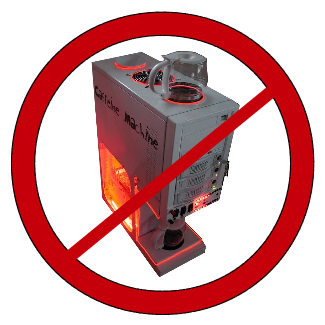
\includegraphics[width=1.3in]{pics/Caffeine_Machine_no_background_red.png}
  \end{itemize}
\end{itemize}
\end{frame}

\frame{
  \frametitle{Faster on CPU and GPU}
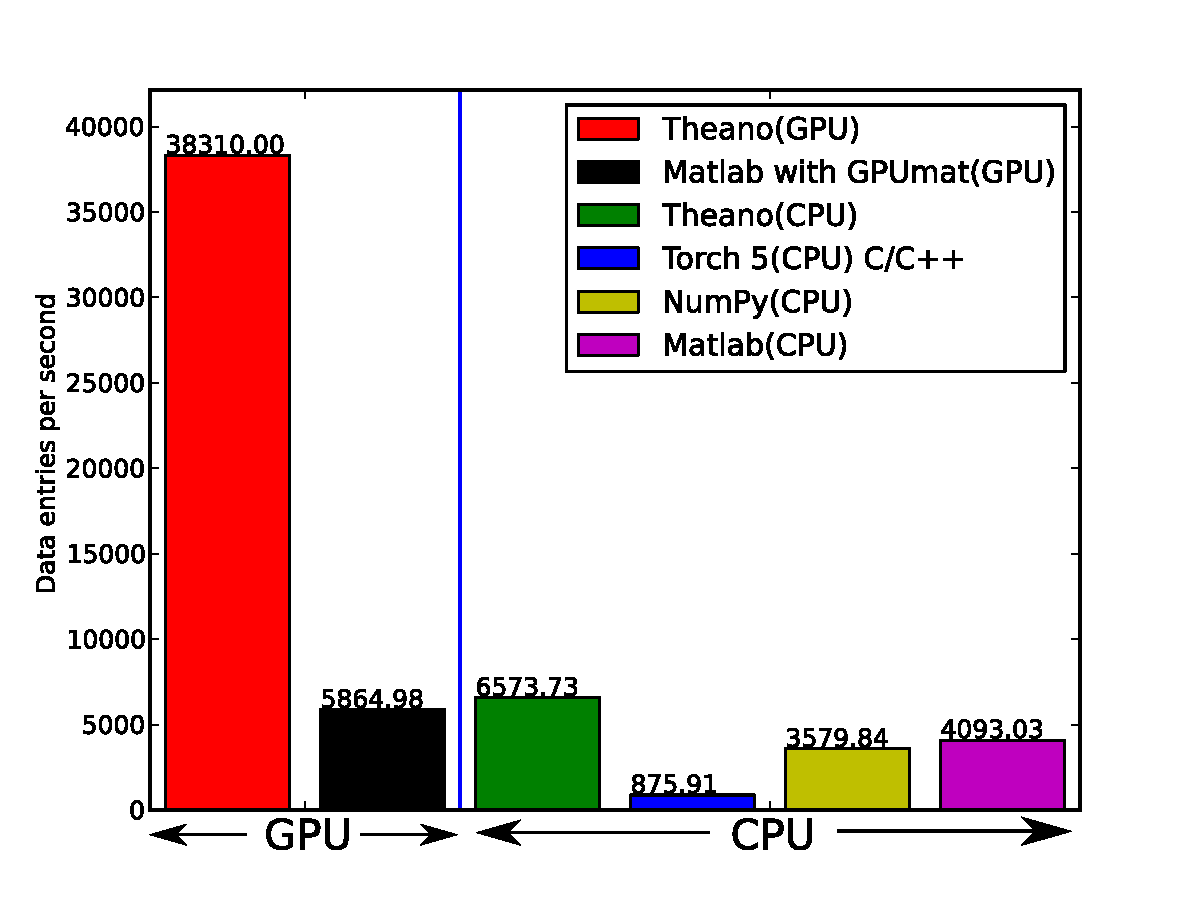
\includegraphics[width=3.in]{pics/mlp.pdf}
}

\frame{
  \frametitle{Project Status}
  Why you can rely on Theano:
  \begin{itemize}  
  \item Theano has been developed and used since January 2008 (3.5 yrs old)
  \item Core technology for a funded Silicon-Valley startup
  \item Driven over 40 research papers in the last few years
  \item Good user documentation
  \item Active mailing list with participants from outside our lab
  \item Many contributors (some from outside our lab)

    \vfill
  \item Used to teach IFT6266 for two years
  \item Used by everyone in our lab (\textasciitilde 30 people)
  \item Deep Learning Tutorials
  \item Unofficial RPMs for Mandriva
  \item Downloads (June 8 2011, since last January):
    \begin{itemize}
      \item Pypi 780
      \item MLOSS: 483
      \item Assembla (``bleeding edge'' repository): unknown
    \end{itemize}
  \end{itemize}
}

\subsection{Overview}
\frame{
  \frametitle{Overview 1}
  \begin{itemize}
  \item {\bf Exercises as we go}
  \item Introduction
    \begin{itemize}
%Why GPU
    \item Why Scripting for GPUs?
    \item Theano vs. PyCUDA vs. PyOpenCL vs. CUDA
%What is your background
    \item Python in 1 slide
    \item NumPy in 1 slide
    \end{itemize}
  \item Theano
    \begin{itemize}
    \item Introduction
    \item Simple example
% gpu for exercices
% Exercises 1 and how to download the files
    \item Real example
% More info on T.grad
% Where are the optimization in the example?
% Exercises 2: logreg\_example.py
    \item Theano Flags
    \item GPU
% Exercises 3: logreg\_example.py on the gpu
    \item Symbolic Variables
    \item Differentiation Details
    \item Benchmarks % MLP, Convolucion, Elemwise
    \end{itemize}
  \item break?
  \end{itemize}
}

\frame{
  \frametitle{Overview 2}
%  \begin{tabular}{lcr}

  \begin{itemize}
  \item Advanced Theano
    \begin{itemize}
    \item Compilation Pipeline
    \item Inplace Optimization
    \item Profiling
%exercises 4: ProfileMode on logreg\_example, CPU vs GPU
    \item Drawing/Printing Theano Graph
    \item Debugging
    \item Scan (For-Loop generalization)
%exercises 5: about scan
    \item Known Limitations
    \end{itemize} %& 
\includegraphics[width=1.in]{pics/theano_logo.png}
  \begin{tabular}{lcr}
    \imagetop{
\includegraphics[width=1.in]{pics/theano_logo.png}}&
    %\imagetop{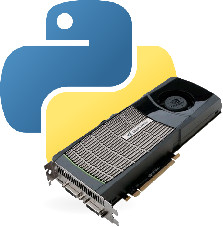
\includegraphics[width=.6in]{pics/pycuda-logo-crop.pdf}}
  \end{tabular}
  \end{itemize}
}

\frame{
  \frametitle{Overview 3}
  \begin{itemize}
  \item PyCUDA
    \begin{itemize}
    \item Introduction
    \item Example
% Exercices 6: pycuda_simple.py
    \end{itemize}
  \item CUDA Overview
  \item Extending Theano
    \begin{itemize}
    \item Theano Graph
    \item Op Contract
    \item Op Example
% Exercises 7: double.py
    \item Theano + PyCUDA
% Exercises 8: pycuda_double_op.py
    \end{itemize}
  \item GpuNdArray
  \item Conclusion
  \end{itemize}
  \begin{tabular}{lcr}
    %\imagetop{
\includegraphics[width=1.in]{pics/theano_logo.png}}&
    \imagetop{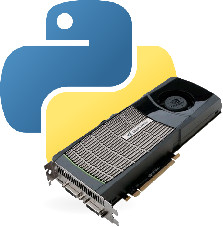
\includegraphics[width=.6in]{pics/pycuda-logo-crop.pdf}}
  \end{tabular} 
}

\frame{
  \frametitle{Overview 4}
  \begin{itemize}
  \item Only high level overview of CUDA
  \item Won't talk about how to optimize GPU code
  \end{itemize}
}

\section{Introduction}
\subsection{Introduction}
\frame{
  \frametitle{Why GPU}
  \begin{itemize}
  \item Faster, cheaper, more efficient power usage
  \item How much faster? I have seen numbers from 100x slower to 1000x faster.
    \begin{itemize}
    \item It depends on the algorithms
    \item How the benchmark is done
      \begin{itemize}
      \item Quality of implementation
      \item How much time was spent optimizing CPU vs GPU code
      \end{itemize}
    \item In Theory: 
      \begin{itemize}
      \item Intel Core i7 980 XE (107Gf/s float64) 6 cores
      \item NVIDIA C2050 (515 Gf/s float64, 1Tf/s float32) 480 cores
      \item NVIDIA GTX580 (1.5Tf/s float32) 512 cores
      \end{itemize}
    \end{itemize}
  \item Theano goes up to 100x faster on th GPU because we don't use multiple core on CPU
    \begin{itemize}
    \item Theano can be linked with multi-core capable BLAS (GEMM and GEMV)
    \end{itemize}
  \item If you see 1000x, it probably means the benchmark is not fair
\end{itemize}

}
\frame{
  \frametitle{Why Scripting for GPUs}
  They {\bf Complement each other}
  \begin{itemize}
  \item GPUs are everything that scripting/high level languages are not
    \begin{itemize}
    \item Highly parallel
    \item Very architecture-sensitive
    \item Built for maximum FP/memory throughput
    \end{itemize}
  \item CPU: largely restricted to control
    \begin{itemize}
    \item Optimized for sequential code and \textit{low latency} (rather than high throughput)
    \item Tasks (1000/sec)
    \item Scripting fast enough
    \end{itemize}
  \end{itemize}
}
\frame{
  \frametitle{Theano vs PyCUDA vs PyOpenCL vs CUDA}
  \begin{itemize}
    \item Theano
      \begin{itemize}
      \item Mathematical expression compiler
      \item Generates costum C and CUDA code
      \item Uses Python code when performance is not critical
      \end{itemize}
    \item CUDA
      \begin{itemize}
      \item C extension by NVIDA that allow to code and use GPU
      \end{itemize}
    \item PyCUDA (Python + CUDA)
      \begin{itemize}
        \item Python interface to CUDA
        \item Memory management of GPU objects
        \item Compilation of code for the low-level driver
      \end{itemize}
    \item PyOpenCL (Python + OpenCL)
      \begin{itemize}
      \item PyCUDA for OpenCL
      \end{itemize}
  \end{itemize}
}

\frame{
  \frametitle{What is your background ?}
  Do you have experience with :
  \begin{itemize}
  \item Python
  \item NumPy / SciPy / Matlab
  \item Maple / Mathematica / SymPy
  \item GPU programming / CUDA / OpenCL
  \item Cython / Weave / Numexpr
  \item C / Java / Fortran
  \end{itemize}
}

\frame{
  \frametitle{Python in 1 Slide}
  \begin{itemize}
    \item Interpreted language
    \item General-purpose high-level programming language
    \item OO and scripting language
    \item Emphasizes code readability
    \item Large and comprehensive standard library
    \item Indentation for block delimiters
    \item Dynamic type and memory management
    \item Dictionary \texttt{d=\{'var1':'value1', 'var2':42, ...\}}
    \item List comprehension: \texttt{[i+3 for i in range(10)]}
  \end{itemize}
}

\frame{
  \frametitle{NumPy in 1 Slide}
  \begin{itemize}
  \item Base scientific computing package in Python on the CPU
  \item A powerful N-dimensional array object
    \begin{itemize}
    \item ndarray.\{ndim, shape, size, dtype, itemsize, stride\}
    \end{itemize}
  \item Sophisticated ``broadcasting'' functions
    \begin{itemize}
    \item \texttt{numpy.random.rand(4,5) * numpy.random.rand(1,5)} $\Rightarrow$ mat(4,5)
    \item \texttt{numpy.random.rand(4,5) * numpy.random.rand(4,1)} $\Rightarrow$ mat(4,5)
    \item \texttt{numpy.random.rand(4,5) * numpy.random.rand(5)} $\Rightarrow$ mat(4,5)
    \end{itemize}
  \item Tools for integrating C/C++ and Fortran code
  \item Linear algebra, Fourier transform and pseudorandom number generation
  \end{itemize}


}

%\frame{
%  \frametitle{Competitors TODO: Remove? Missing many I think!}
%  There are some competitors for easy computing on gpu.
%  \begin{itemize}
%  \item Jacket(GPU for matlab): http://www.accelereyes.com/
%  \item GPUmat(GPU for matlab, free): http://gp-you.org/
%  \item numexpr, algopy
%  \end{itemize}
%}

\section{Theano}
\subsection{Introduction}
\frame{
%%  \frametitle{Theano}
\begin{center}
  
\includegraphics[width=3.in]{../images/theano_logo_allblue_350x95.png}
%  
\includegraphics[width=3.in]{../images/theano_logo_allblue_200x54.png}
\end{center}
}

\frame{
  \frametitle{Pointers}
  \begin{itemize}
  \item Website: http://deeplearning.net/software/theano/
  \item Announcements mailing list: http://groups.google.com/group/theano-announce
  \item User mailing list: http://groups.google.com/group/theano-users
  \item Deep Learning Tutorials: http://www.deeplearning.net/tutorial/

    \vfill 
  \item Installation: https://deeplearning.net/software/theano/install.html
  \end{itemize}
}

\frame{
  \frametitle{Description}
  \begin{itemize}
  \item Mathematical symbolic expression compiler
  \item Dynamic C/CUDA code generation
  \item Efficient symbolic differentiation
    \begin{itemize}
    \item Theano computes derivatives of functions with one or many inputs.
    \end{itemize}
  \item Speed and stability optimizations 
    \begin{itemize}
    \item Gives the right answer for $\log(1+x)$ even if x is really tiny.
    \end{itemize}
  \item Works on Linux, Mac and Windows
  \item Transparent use of a GPU
    \begin{itemize}
    \item float32 only for now (working on other data types)
    \item Doesn't work on Windows for now
    \item On GPU data-intensive calculations are typically between 6.5x and 44x faster. We've seen speedups up to 140x
    \end{itemize}  \end{itemize}
}

\frame{
  \frametitle{Description 2}
  \begin{itemize}    
  \item Extensive unit-testing and self-verification
    \begin{itemize}
    \item Detects and diagnoses many types of errors
    \end{itemize}
  \item On CPU, common machine learning algorithms are 1.6x to 7.5x faster than competitive alternatives 
    \begin{itemize}
    \item including specialized implementations in C/C++, NumPy, SciPy, and Matlab
    \end{itemize}
  \item Expressions mimic NumPy's syntax \& semantics
  \item Statically typed and purely functional
  \item Some sparse operations (CPU only)
  \item The project was started by James Bergstra and Olivier Breuleux
  \item For the past 1-2 years, I have replaced Olivier as lead contributor
  \end{itemize}
}

\frame{
  \frametitle{Why Theano is better}
  Executing the code is faster because Theano:
  \begin{itemize}
  \item Rearranges high-level expressions 
  \item Produces customized low-level code
  \item Uses a variety of backend technologies (GPU,...)
  \end{itemize}

  \vfill
  Writing the code is faster because:
  \begin{itemize}
  \item High-level language allows to {\bf concentrate on the algorithm}
  \item Theano do {\bf automatic optimization}
    \begin{itemize}
    \item No need to manually optimize for each algorithm you want to test
    \end{itemize}
  \item Theano do {\bf automatic efficient symbolic differentiation}
    \begin{itemize}
    \item No need to manually differentiate your functions (tedious \& error-prone for complicated expressions!)
    \end{itemize}    
  \end{itemize}
}

\newcommand\codeHighlight[1]{\textcolor[rgb]{1,0,0}{\textbf{#1}}}
\subsection{Simple Example}

\begin{frame}[fragile]
  \frametitle{Simple Example}
\begin{Verbatim}[commandchars=\\\{\}]
import theano
a = theano.tensor.vector("a") {\color{gray} # declare symbolic variable}
b = a + a**10                 {\color{gray} # build symbolic expression}
f = theano.function([a], b)   {\color{gray} # compile function}
print f([0,1,2])              {\color{gray} # prints `array([0,2,1026])`}
\end{Verbatim}
  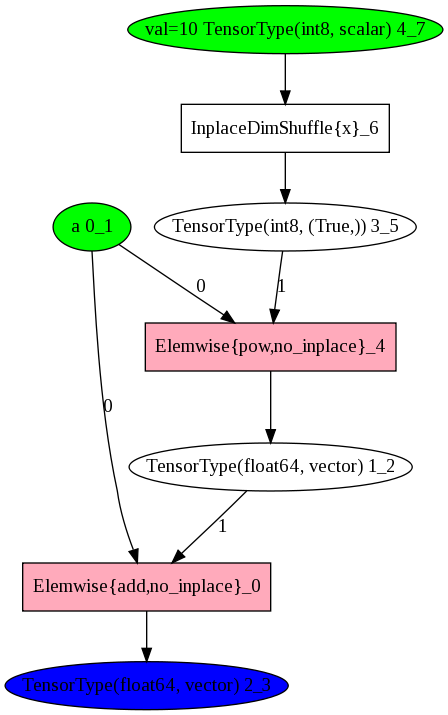
\includegraphics[width=1.2in]{pics/f_unoptimized.png}
\end{frame}

\frame{
  \frametitle{Simple Example: Optimized graph}
             {\bf no pow, fused elemwise op!}

  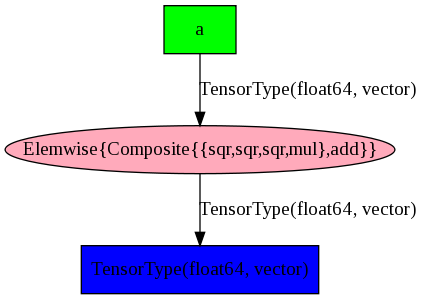
\includegraphics[width=2.3in]{pics/f_optimized.png}

  Symbolic programming
  \begin{itemize}
  \item Paradigm shift: people need to use it to understand it
  \end{itemize}
}

\begin{frame}[fragile]
  \frametitle{Exercises 1}
  \begin{Verbatim}
source /groups/h/hpc2011/bin/GPU.csh
hg clone http://hg.assembla.com/theano Theano
cd Theano/doc/hpcs2011_tutorial
python simple_example.py
  \end{Verbatim}
  \vfill
Modify and execute the example to do this expression: a**2 + b**2 + 2*a*b
\end{frame}

\subsection{Real Example}
\frame{
  \frametitle{A Real Example: Logistic Regression}
  \begin{itemize}
  \item GPU-ready
  \item Symbolic differentiation
  \item Speed optimizations
  \item Stability optimizations
  \end{itemize}
}

\begin{frame}[fragile]
  \frametitle{A Real Example: Logistic Regression}
\begin{Verbatim}[commandchars=\\\{\}]
import numpy
import theano
import theano.tensor as T
rng = numpy.random

N = 400
feats = 784
D = (rng.randn(N, feats), rng.randint(size=N,low=0, high=2))
training_steps = 10000
\end{Verbatim}
\end{frame}

\begin{frame}[fragile]
  \frametitle{A Real Example: Logistic Regression}
\begin{Verbatim}[commandchars=\\\{\}]
{\color{gray}# Declare Theano symbolic variables}
x = T.matrix("x")
y = T.vector("y")
\codeHighlight{w = theano.shared(rng.randn(100), name="w")}
\codeHighlight{b = theano.shared(0., name="b")}
print "Initial model:"
print w.get_value(), b.get_value()
\end{Verbatim}
\end{frame}

\begin{frame}[fragile]
  \frametitle{A Real Example: Logistic Regression}
\begin{Verbatim}[commandchars=\\\{\}]
{\color{gray}# Declare Theano symbolic variables}
{\color{gray}x = T.matrix("x")}
{\color{gray}y = T.vector("y")}
{\color{gray}w = theano.shared(rng.randn(100), name="w")}
{\color{gray}b = theano.shared(0., name="b")}

{\color{gray}# Construct Theano expression graph}
p_1 = 1 / (1 + T.exp(-T.dot(x, w)-b))    {\color{gray}# Probability that target = 1}
prediction = p_1 > 0.5                   {\color{gray}# The prediction thresholded}
xent = -y*T.log(p_1) - (1-y)*T.log(1-p_1){\color{gray}# Cross-entropy loss function}
cost = xent.mean() + 0.01*(w**2).sum()   {\color{gray}# The cost to minimize}
\codeHighlight{gw,gb = T.grad(cost, [w,b])}
\end{Verbatim}
\end{frame}

\begin{frame}[fragile]
  \frametitle{A Real Example: Logistic Regression}
\begin{Verbatim}[commandchars=\\\{\}]
{\color{gray}x = T.matrix("x")}
{\color{gray}y = T.vector("y")}
{\color{gray}w = theano.shared(rng.randn(100), name="w")}
{\color{gray}b = theano.shared(0., name="b")}
{\color{gray}p_1 = 1 / (1 + T.exp(-T.dot(x, w)-b))}
{\color{gray}prediction = p_1 > 0.5}
{\color{gray}xent = -y*T.log(p_1) - (1-y)*T.log(1-p_1)}
{\color{gray}cost = xent.mean() + 0.01*(w**2).sum()}
{\color{gray}gw,gb = T.grad(cost, [w,b])}

{\color{gray}# Compile}
train = theano.function(
            inputs=[x,y],
            \codeHighlight{outputs=[prediction, xent]},
            \codeHighlight{updates=\{w:w-0.1*gw, b:b-0.1*gb\}})
predict = theano.function(inputs=[x], outputs=prediction)
\end{Verbatim}
\end{frame}

\begin{frame}[fragile]
  \frametitle{A Real Example: Logistic Regression}
\begin{Verbatim}[commandchars=\\\{\}]
{\color{gray}# Train}
for i in range(training_steps):
    pred, err = train(D[0], D[1])

print "Final model:"
print w.get_value(), b.get_value()
print "target values for D:", D[1]
print "prediction on D:", predict(D[0])
\end{Verbatim}
\end{frame}

\begin{frame}[fragile]
  \frametitle{A Real Example: optimization}
\begin{Verbatim}[commandchars=\\\{\}]
p_1 = 1 / (1 + T.exp(-T.dot(x, w)-b))
xent = -y*T.log(p_1) - (1-y)*T.log(1-p_1)
prediction = p_1 > 0.5
cost = xent.mean() + 0.01*(w**2).sum()
gw,gb = T.grad(cost, [w,b])

train = theano.function(
            inputs=[x,y],
            outputs=[prediction, xent],
            updates=\{w:w-0.1*gw, b:b-0.1*gb\})  {\color{gray}# This is a dictionary}
\end{Verbatim}
Where are those optimization applied?
\begin{itemize}
\item Log(1+exp(x))
\item 1 / (1 + T.exp(var)) (sigmoid)
\item Log(1-sigmoid(var)) (softplus, stabilisation)
\item GEMV (matrix-vector multiply from BLAS)
\item Loop fusion
\end{itemize}
\end{frame}

\begin{frame}[fragile]
  \frametitle{A Real Example: optimization!}
\begin{Verbatim}[commandchars=\\\{\}]
p_1 = 1 / (1 + T.exp(-T.dot(x, w)-b))
\codeHighlight{# 1 / (1 + T.exp(var)) -> sigmoid(var)}
xent = -y*T.log(p_1) - (1-y)*T.log(1-p_1)
\codeHighlight{# Log(1-sigmoid(var)) -> -sigmoid(var)}

prediction = p_1 > 0.5
cost = xent.mean() + 0.01*(w**2).sum()
gw,gb = T.grad(cost, [w,b])

train = theano.function(
            inputs=[x,y],
            outputs=[prediction, xent],
\codeHighlight{# w-0.1*gw: GEMV with the dot in the grad}
            updates=\{w:w-0.1*gw, b:b-0.1*gb\})

\end{Verbatim}
\begin{itemize}
\item Loop fusion in many places
\end{itemize}
\end{frame}

\subsection{Theano Flags}
\frame{
\frametitle{Theano Flags}
Theano can be configured with flags. They can be defined in two ways
\begin{itemize}
\item With an environment variable: \texttt{THEANO\_FLAGS="mode=ProfileMode,ProfileMode.profile\_memory=True"}
\item With a configuration file that defaults to \textasciitilde/.theanorc
\end{itemize}
}

\begin{frame}[fragile]
\frametitle{Exercises 2}
\begin{Verbatim}
python logreg_example.py
\end{Verbatim}
\vfill
Modify and execute the example in the file logreg\_example.py to run on CPU with floatX=float32

* You will need to use: theano.config.floatX and ndarray.astype("str")
\end{frame}

\subsection{GPU}
\frame{
\frametitle{GPU}
\begin{itemize}
\item Only 32 bit floats are supported (being worked on)
\item Only 1 GPU per process
\item Use the Theano flag \texttt{device=gpu} to tell to use the GPU device
  \begin{itemize}
  \item Use \texttt{device=gpu{0, 1, ...}} to specify which GPU if you have more than one
  \item Shared variables with float32 dtype are by default moved to the GPU memory space
  \end{itemize}
\item Use the Theano flag \texttt{floatX=float32}
  \begin{itemize}
  \item Be sure to use \texttt{floatX} (\texttt{theano.config.floatX}) in your code
  \item Cast inputs before putting them into a shared variable
  \item Cast "problem": int32 with float32 $\to$ float64
    \begin{itemize}    
    \item A new casting mechanism is being developed
    \item Insert manual cast in your code or use [u]int{8,16}
    \item Insert manual cast around the mean operator (which involves a division by the length, which is an int64!)
    \end{itemize}
  \end{itemize}
\end{itemize}
}

\frame{
\frametitle{GPU for Exercises}
\begin{itemize}
\item Intel Core i7 980 XE (107Gf/s float64, 1050\$, 6 cores/12 threads)
\item NVIDIA C2050 (515 Gf/s float64, 1Tf/s float32, 2400\$, 480 cores), compute capability 2.0
\item NVIDIA GTX580 (1.5Tf/s float32, 500\$, 512 cores), compute capability 2.0
\end{itemize}
Computers in the class
\begin{itemize}
\item Intel Xeon X3450 (?56? flops/s, 383\$, 4 cores)
\item NVIDIA Quadro FX 580 (71GF/s single, 140\$, 32 cores), compute capability 1.1, 'profesionnal card'
% BLAS on the cpu took 48s, 4s on the GPU
\end{itemize}

%Device 0: "Quadro FX 580"
% Total amount of global memory:                 536150016 bytes
% Multiprocessors x Cores/MP = Cores:            4 (MP) x 8 (Cores/MP) = 32 (Cores)
% Clock rate:                                    1.12 GHz
% Run time limit on kernels:                     Yes
% Compute mode:                                  Default (multiple host
%threads can use this device simultaneously)
}

\begin{frame}
\frametitle{Exercises 3}

\begin{itemize}
\item Modify and execute the code to run with floatX=float32 on GPU
\item Time with: \texttt{time python file.py}
\end{itemize}
\end{frame}

\subsection{Symbolic Variables}
\frame{
  \frametitle{Creating symbolic variables}
  \begin{itemize}
  \item \# Dimensions
    \begin{itemize}
    \item T.scalar, T.vector, T.matrix, T.tensor3, T.tensor4
    \end{itemize}
  \item Dtype
    \begin{itemize}
    \item T.[fdczbwil]vector (float32, float64, complex64, complex128, int8, int16, int32, int64)
    \item T.vector $\to$ floatX dtype
    \item floatX: configurable dtype that can be float32 or float64.
    \end{itemize}
  
  \item Custom variable
    \begin{itemize}
    \item All are shortcuts to: T.tensor(dtype, broadcastable=[False]*nd)
    \item Other dtype: uint[8,16,32,64], floatX
    \end{itemize}
  \end{itemize}
}

\frame{
  \frametitle{Creating symbolic variables: Broadcastability}
  \begin{itemize}
  \item Remember what I said about broadcasting? 
  \item How to add a row to all rows of a matrix? 
  \item How to add a column to all columns of a matrix? 
  \end{itemize}
  \vfill
  \begin{itemize}
  \item Broadcastability must be specified when creating the variable
  \item The only shorcut with broadcastable dimensions are: {\bf T.row} and {\bf T.col}
  \item For all others: T.tensor(dtype, broadcastable={\bf ([False or True])*nd})
  \end{itemize}
}

\subsection{Differentiation Details}
\begin{frame}[fragile]
  \frametitle{Differentiation Details}
\begin{Verbatim}[commandchars=\\\{\}]
{\color{gray}gw,gb = T.grad(cost, [w,b])}
\end{Verbatim}
\begin{itemize}
\item T.grad works symbolically: takes and returns a Theano variable
\item T.grad can be compared to a macro: it can be applied multiple times
\item T.grad takes scalar costs only
\item Simple recipe allows to compute efficiently vector $\times$ Jacobian and vector $\times$ Hessian
\item We are working on the missing optimizations to be able to compute efficently the full Jacobian and Hessian and Jacobian $\times$ vector
\end{itemize}
\end{frame}

\subsection{Benchmarks}
\frame{
\frametitle{Benchmarks}
Example:
\begin{itemize}
\item Multi-layer perceptron
\item Convolutional Neural Networks
\item Misc Elemwise operations
\end{itemize}

Competitors: NumPy + SciPy, MATLAB, EBLearn, Torch5, numexpr
\begin{itemize}
\item EBLearn, Torch5: specialized libraries written by practitioners specifically for these tasks
\item numexpr: similar to Theano, 'virtual machine' for elemwise expressions
\end{itemize}
}

\frame{
\frametitle{Benchmark MLP}
Multi-Layer Perceptron: 60x784 matrix times 784x500 matrix, tanh, times 500x10 matrix, elemwise, then all in reverse for backpropagation
\begin{center}
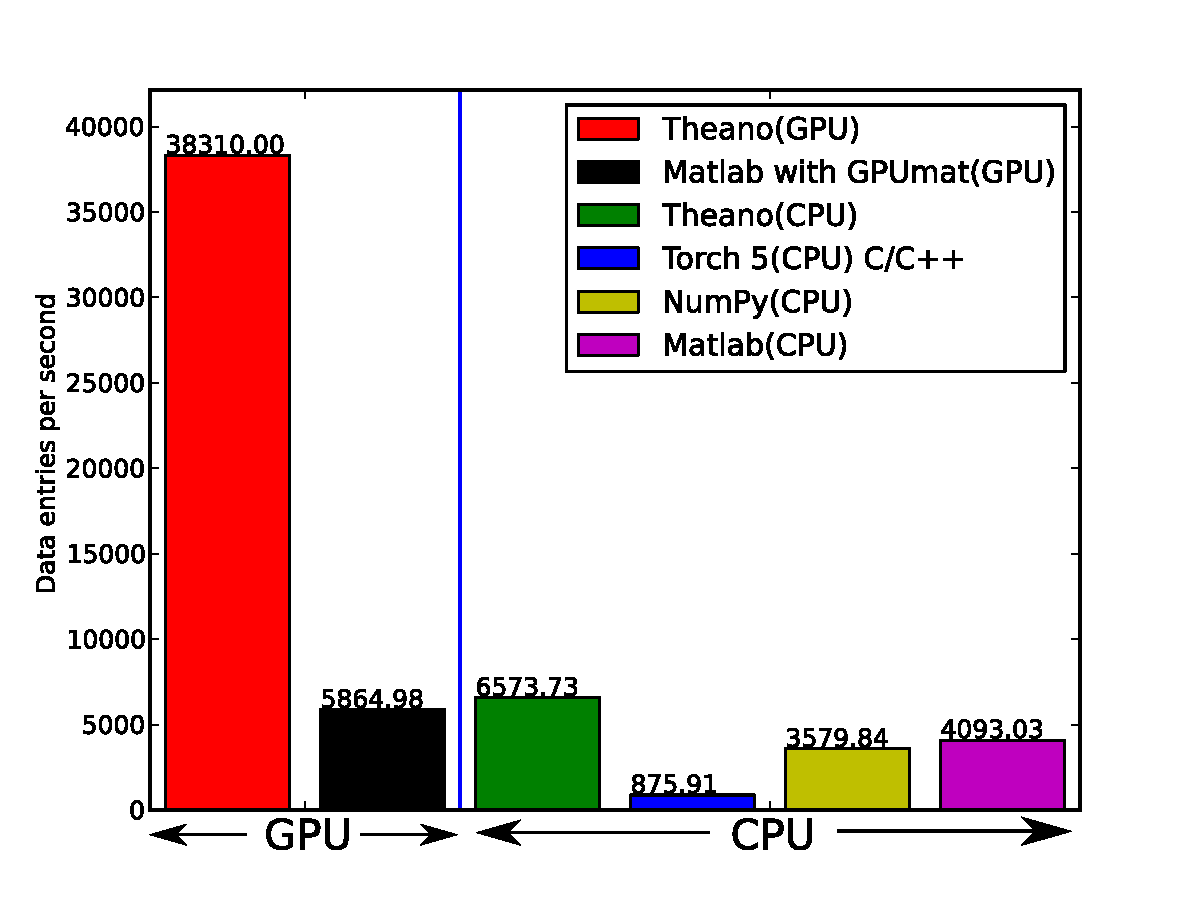
\includegraphics[width=3.in]{pics/mlp.pdf}
\end{center}

}

\frame{
\frametitle{Benchmark Convolutional Network}
Convolutional Network: 256x256 images convolved with 6 7x7 filters, downsampled to 6x50x50, tanh, convolution with 16 6x7x7 filter, elementwise tanh, matrix multiply, softmax elementwise, then in reverse
\begin{center}
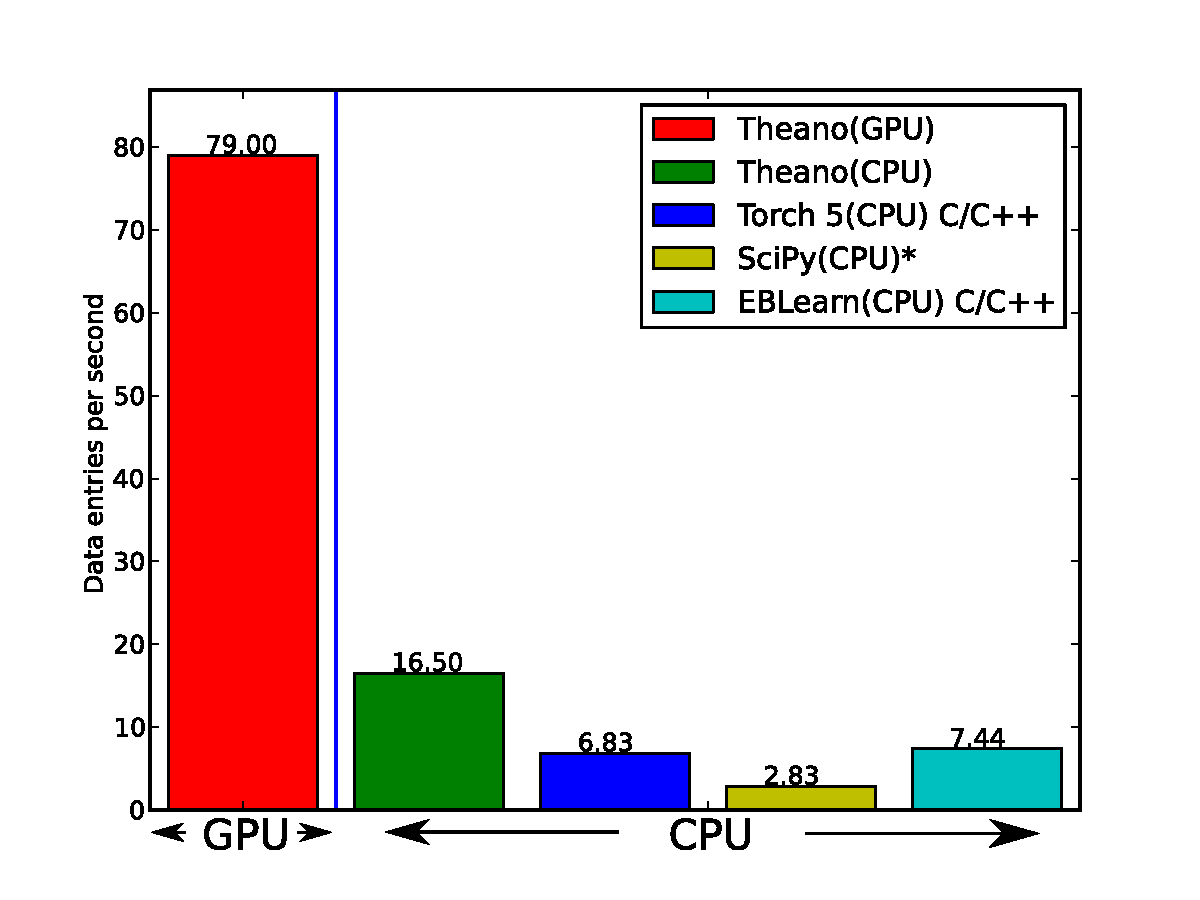
\includegraphics[width=3.in]{pics/conv.pdf}
\end{center}
}

\frame{
\frametitle{Elemwise Benchmark}
\begin{itemize}
\item All on CPU
\item Solid blue: Theano
\item Dashed Red: numexpr (without MKL)
\end{itemize}
\begin{center}
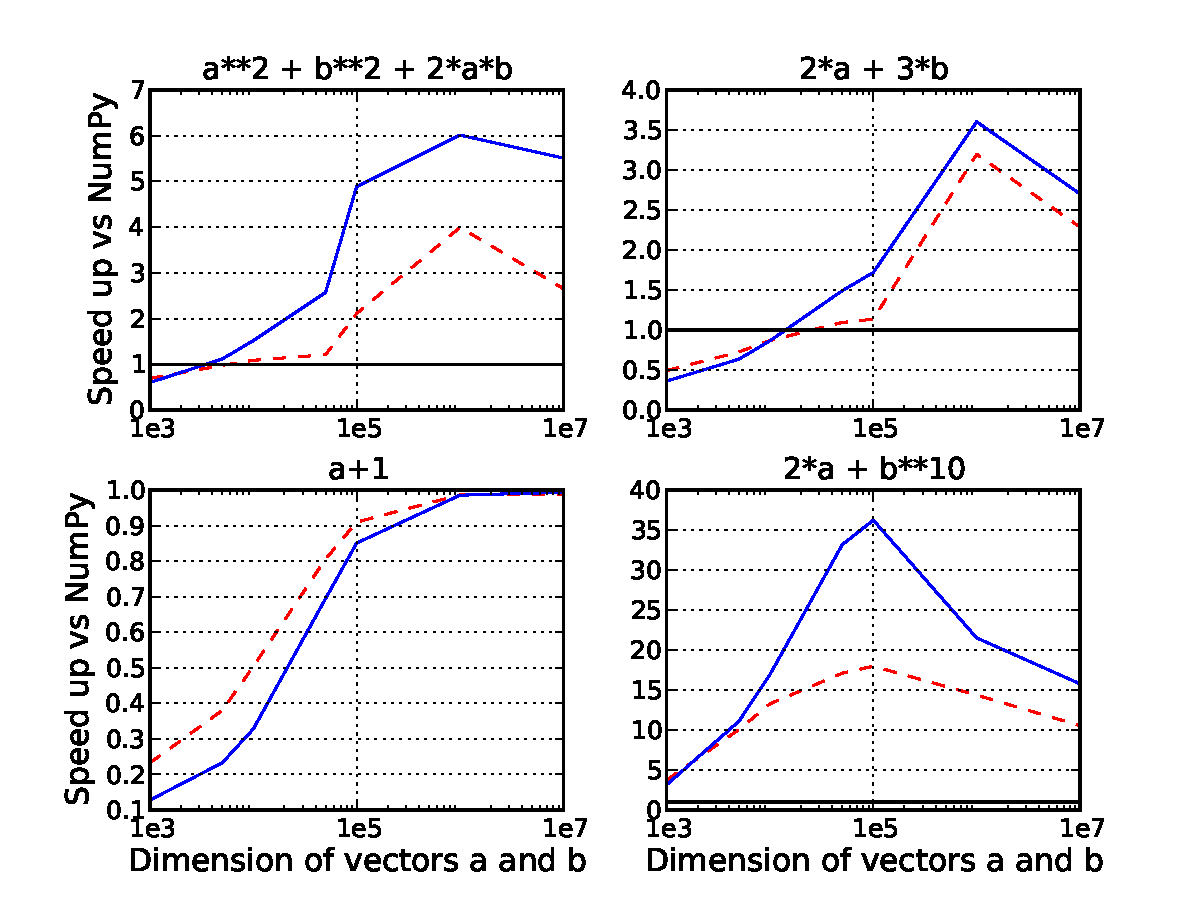
\includegraphics[width=2.8in]{pics/multiple_graph.pdf}
\end{center}
}

\section{Advanced Theano}
\subsection{Optimizations}
\frame{
\frametitle{Compilation Pipeline}
\begin{center}
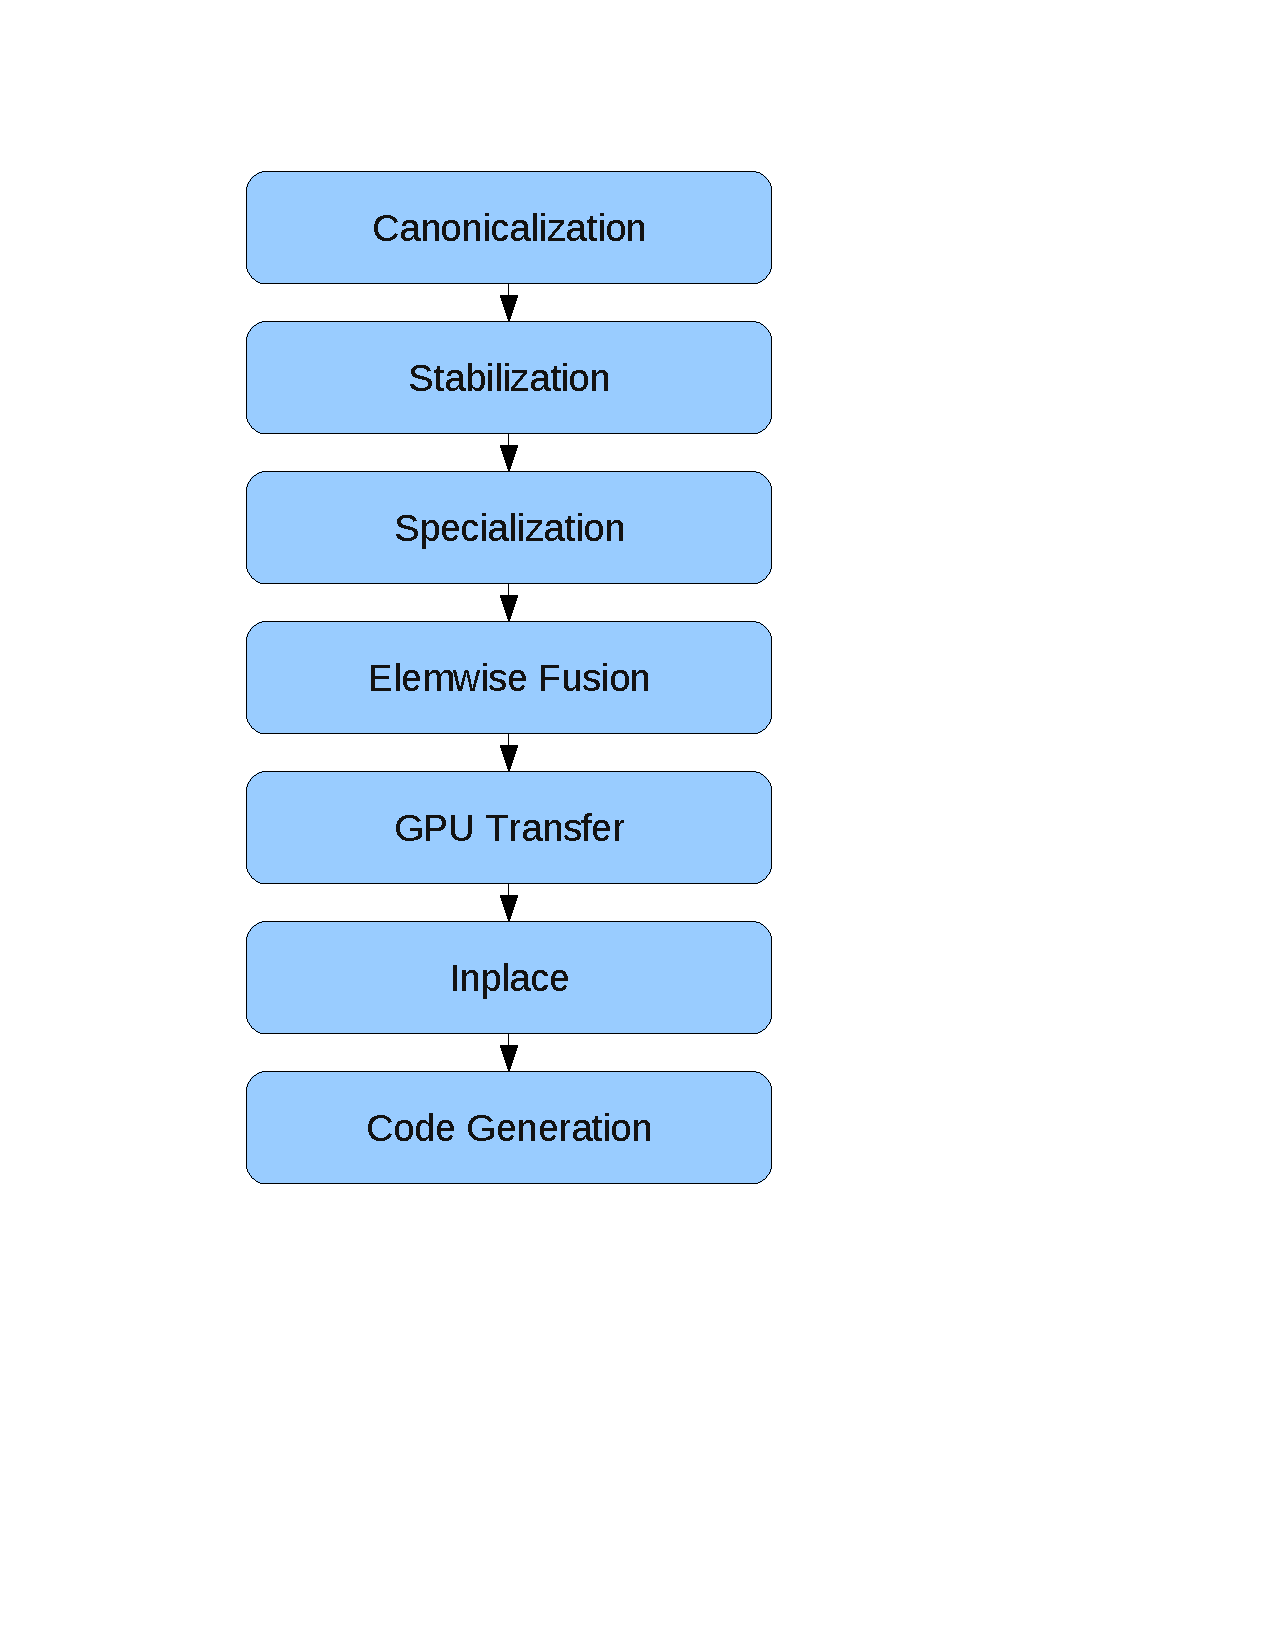
\includegraphics[width=2.7in]{pics/pipeline.pdf}
\end{center}
}

\frame{
\frametitle{Inplace Optimization}
\begin{itemize}
\item 2 type of inplace operations:
  \begin{itemize}
  \item An op that return a view on its inputs (e.g. reshape, inplace transpose)
  \item An op that write the output on the inputs memory space
  \end{itemize}
\item This allows some memory optimization
\item The Op must tell Theano if they work inplace
\item Inplace Op add constraints to the order of execution
\end{itemize}
}

\subsection{Profiling}
\begin{frame}[fragile]
\frametitle{Profile Mode}
To replace the default mode with this mode, use the Theano flags \texttt{mode=ProfileMode}

To enable the memory profiling use the flags \texttt{ProfileMode.profile\_memory=True} 
\begin{Verbatim}
Time since import 33.456s
Theano compile time: 1.023s (3.1% since import)
    Optimization time: 0.789s
    Linker time: 0.221s
Theano fct call 30.878s (92.3% since import)
   Theano Op time 29.411s 87.9%(since import) 95.3%(of fct call)
   Theano function overhead in ProfileMode 1.466s 4.4%(since import)
                                                  4.7%(of fct call)
10001 Theano fct call, 0.003s per call
Rest of the time since import 1.555s 4.6%
\end{Verbatim}
\end{frame}

\begin{frame}[fragile]
\frametitle{Profile Mode: Function Summary}
Theano outputs:
\vfill
\begin{Verbatim}
Theano fct summary:
<% total fct time> <total time> <time per call> <nb call> <fct name>
   100.0% 30.877s 3.09e-03s 10000 train
    0.0% 0.000s 4.06e-04s 1 predict
\end{Verbatim}
\end{frame}

\begin{frame}[fragile]
\frametitle{Profile Mode: Single Op-Wise Summary}
Theano outputs:
\vfill
\begin{Verbatim}
Single Op-wise summary:
<% of local_time spent on this kind of Op> <cumulative %> 
    <self seconds> <cumulative seconds> <time per call> <nb_call>
    <nb_op> <nb_apply> <Op name>
   87.3%   87.3%  25.672s  25.672s  2.57e-03s   10000  1  1 <Gemv>
    9.7%   97.0%  2.843s  28.515s  2.84e-04s   10001  1  2 <Dot>
    2.4%   99.3%  0.691s  29.206s  7.68e-06s * 90001 10 10 <Elemwise>
    0.4%   99.7%  0.127s  29.334s  1.27e-05s   10000  1  1 <Alloc>
    0.2%   99.9%  0.053s  29.386s  1.75e-06s * 30001  2  4 <DimShuffle>
    0.0%  100.0%  0.014s  29.400s  1.40e-06s * 10000  1  1 <Sum>
    0.0%  100.0%  0.011s  29.411s  1.10e-06s * 10000  1  1 <Shape_i>
(*) Op is running a c implementation
\end{Verbatim}
\end{frame}

\begin{frame}[fragile]
\frametitle{Profile Mode: Op-Wise Summary}
Theano outputs:
\vfill
\begin{Verbatim}
Op-wise summary:
<% of local_time spent on this kind of Op> <cumulative %>
    <self seconds> <cumulative seconds> <time per call>
    <nb_call> <nb apply> <Op name>
   87.3%   87.3%  25.672s  25.672s  2.57e-03s   10000  1 Gemv{inplace}
    9.7%   97.0%  2.843s  28.515s  2.84e-04s   10001  2 dot
    1.3%   98.2%  0.378s  28.893s  3.78e-05s * 10000  1 Elemwise{Composite{
        scalar_softplus,{mul,scalar_softplus,{neg,mul,sub}}}}
    0.4%   98.7%  0.127s  29.021s  1.27e-05s   10000  1 Alloc
    0.3%   99.0%  0.092s  29.112s  9.16e-06s * 10000  1 Elemwise{Composite{
        exp,{mul,{true_div,neg,{add,mul}}}}}[(0, 0)]
    0.1%   99.3%  0.033s  29.265s  1.66e-06s * 20001  3 InplaceDimShuffle{x}
   ... (remaining 11 Apply account for 0.7%(0.00s) of the runtime)
(*) Op is running a c implementation
\end{Verbatim}
\end{frame}

\begin{frame}[fragile]
\frametitle{Profile Mode: Apply-Wise Summary}
Theano outputs:
\vfill
\begin{Verbatim}
Apply-wise summary:
<% of local_time spent at this position> <cumulative %%>
    <apply time> <cumulative seconds> <time per call>
    <nb_call> <Apply position> <Apply Op name>
   87.3%   87.3%  25.672s  25.672s 2.57e-03s  10000  15 Gemv{inplace}(
        w, TensorConstant{-0.01}, InplaceDimShuffle{1,0}.0, Elemwise{Composite{exp,{mul,{true_div,neg,{add,mul}}}}}[(0, 0)].0, TensorConstant{0.9998})
    9.7%   97.0%  2.843s  28.515s 2.84e-04s  10000   1 dot(x, w)
    1.3%   98.2%  0.378s  28.893s 3.78e-05s  10000   9 Elemwise{Composite{scalar_softplus,{mul,scalar_softplus,{neg,mul,sub}}}}(y, Elemwise{Composite{neg,sub}}[(0, 0)].0, Elemwise{sub,no_inplace}.0, Elemwise{neg,no_inplace}.0)
    0.4%   98.7%  0.127s  29.020s 1.27e-05s  10000  10 Alloc(Elemwise{inv,no_inplace}.0, Shape_i{0}.0)
    0.3%   99.0%  0.092s  29.112s 9.16e-06s  10000  13 Elemwise{Composite{exp,{mul,{true_div,neg,{add,mul}}}}}[(0, 0)](Elemwise{ScalarSigmoid{output_types_preference=transfer_type{0}, _op_use_c_code=True}}[(0, 0)].0, Alloc.0, y, Elemwise{Composite{neg,sub}}[(0, 0)].0, Elemwise{sub,no_inplace}.0, InplaceDimShuffle{x}.0)
    0.3%   99.3%  0.080s  29.192s 7.99e-06s  10000  11 Elemwise{ScalarSigmoid{output_types_preference=transfer_type{0}, _op_use_c_code=True}}[(0, 0)](Elemwise{neg,no_inplace}.0)
   ... (remaining 14 Apply instances account for 
       0.7%(0.00s) of the runtime)
\end{Verbatim}
\end{frame}

\begin{frame}[fragile]
\frametitle{Profile Mode: Memory Profile}
Theano outputs:
\vfill
\begin{Verbatim}
Profile of Theano functions memory:
(This check only the output of each apply node. It don't check the 
    temporary memory used by the op in the apply node.)
Theano fct: train
    Max without gc, inplace and view (KB) 2481
    Max FAST_RUN_NO_GC (KB) 16
    Max FAST_RUN (KB) 16
    Memory saved by view (KB) 2450
    Memory saved by inplace (KB) 15
    Memory saved by GC (KB) 0
    <Sum apply outputs (bytes)> <Apply outputs memory size(bytes)> 
        <created/inplace/view> <Apply node>
    <created/inplace/view> is taked from the op declaration, not ...
         2508800B  [2508800] v InplaceDimShuffle{1,0}(x)
            6272B  [6272] i Gemv{inplace}(w, ...)
            3200B  [3200] c Elemwise{Composite{...}}(y, ...)
\end{Verbatim}
\end{frame}

\begin{frame}[fragile]
\frametitle{Profile Mode: Tips}
Theano outputs:
\vfill
\begin{Verbatim}
Here are tips to potentially make your code run faster
(if you think of new ones, suggest them on the mailing list).
Test them first, as they are not guaranteed to always provide a speedup.
  - Try the Theano flag floatX=float32
\end{Verbatim}
\end{frame}

\begin{frame}
\frametitle{Exercises 4}

\begin{itemize}
\item In the last exercises, do you see a speed up with the GPU?
\item Where does it come from? (Use ProfileMode)
\item Is there something we can do to speed up the GPU version?
\end{itemize}
\end{frame}


\subsection{Printing}
\begin{frame}[fragile]
\frametitle{Text Printing of Your Theano Graph: Pretty Printing}
theano.printing.pprint(variable)
\vfill
\begin{Verbatim}
>>> theano.printing.pprint(prediction)
gt((TensorConstant{1} / (TensorConstant{1} + exp(((-(x \\dot w)) - b)))),
TensorConstant{0.5})
\end{Verbatim}
\end{frame}


\begin{frame}[fragile]
\frametitle{Text Printing of Your Theano Graph: Debug Print}
theano.printing.debugprint({fct, variable, list of variables})
\vfill
\small
\begin{Verbatim}
>>> theano.printing.debugprint(prediction)
Elemwise{gt,no_inplace} [@181772236] ''   
 |Elemwise{true_div,no_inplace} [@181746668] ''   
 | |InplaceDimShuffle{x} [@181746412] ''   
 | | |TensorConstant{1} [@181745836]
 | |Elemwise{add,no_inplace} [@181745644] ''   
 | | |InplaceDimShuffle{x} [@181745420] ''   
 | | | |TensorConstant{1} [@181744844]
 | | |Elemwise{exp,no_inplace} [@181744652] ''   
 | | | |Elemwise{sub,no_inplace} [@181744012] ''   
 | | | | |Elemwise{neg,no_inplace} [@181730764] ''   
 | | | | | |dot [@181729676] ''   
 | | | | | | |x [@181563948]
 | | | | | | |w [@181729964]
 | | | | |InplaceDimShuffle{x} [@181743788] ''   
 | | | | | |b [@181730156]
 |InplaceDimShuffle{x} [@181771788] ''   
 | |TensorConstant{0.5} [@181771148]
\end{Verbatim}
\end{frame}

\begin{frame}[fragile]
\frametitle{Text Printing of Your Theano Graph: Debug Print}
theano.printing.debugprint({fct, variable, list of variables})
\vfill
\small
\begin{Verbatim}
>>> theano.printing.debugprint(predict)
Elemwise{Composite{neg,{sub,{{scalar_sigmoid,GT},neg}}}} [@183160204] ''   2
 |dot [@183018796] ''   1
 | |x [@183000780]
 | |w [@183000812]
 |InplaceDimShuffle{x} [@183133580] ''   0
 | |b [@183000876]
 |TensorConstant{[ 0.5]} [@183084108]
\end{Verbatim}
\end{frame}

\begin{frame}[fragile]
\frametitle{Picture Printing of Graphs}
\begin{Verbatim}
>>> theano.printing.pydotprint_variables(prediction)
\end{Verbatim}
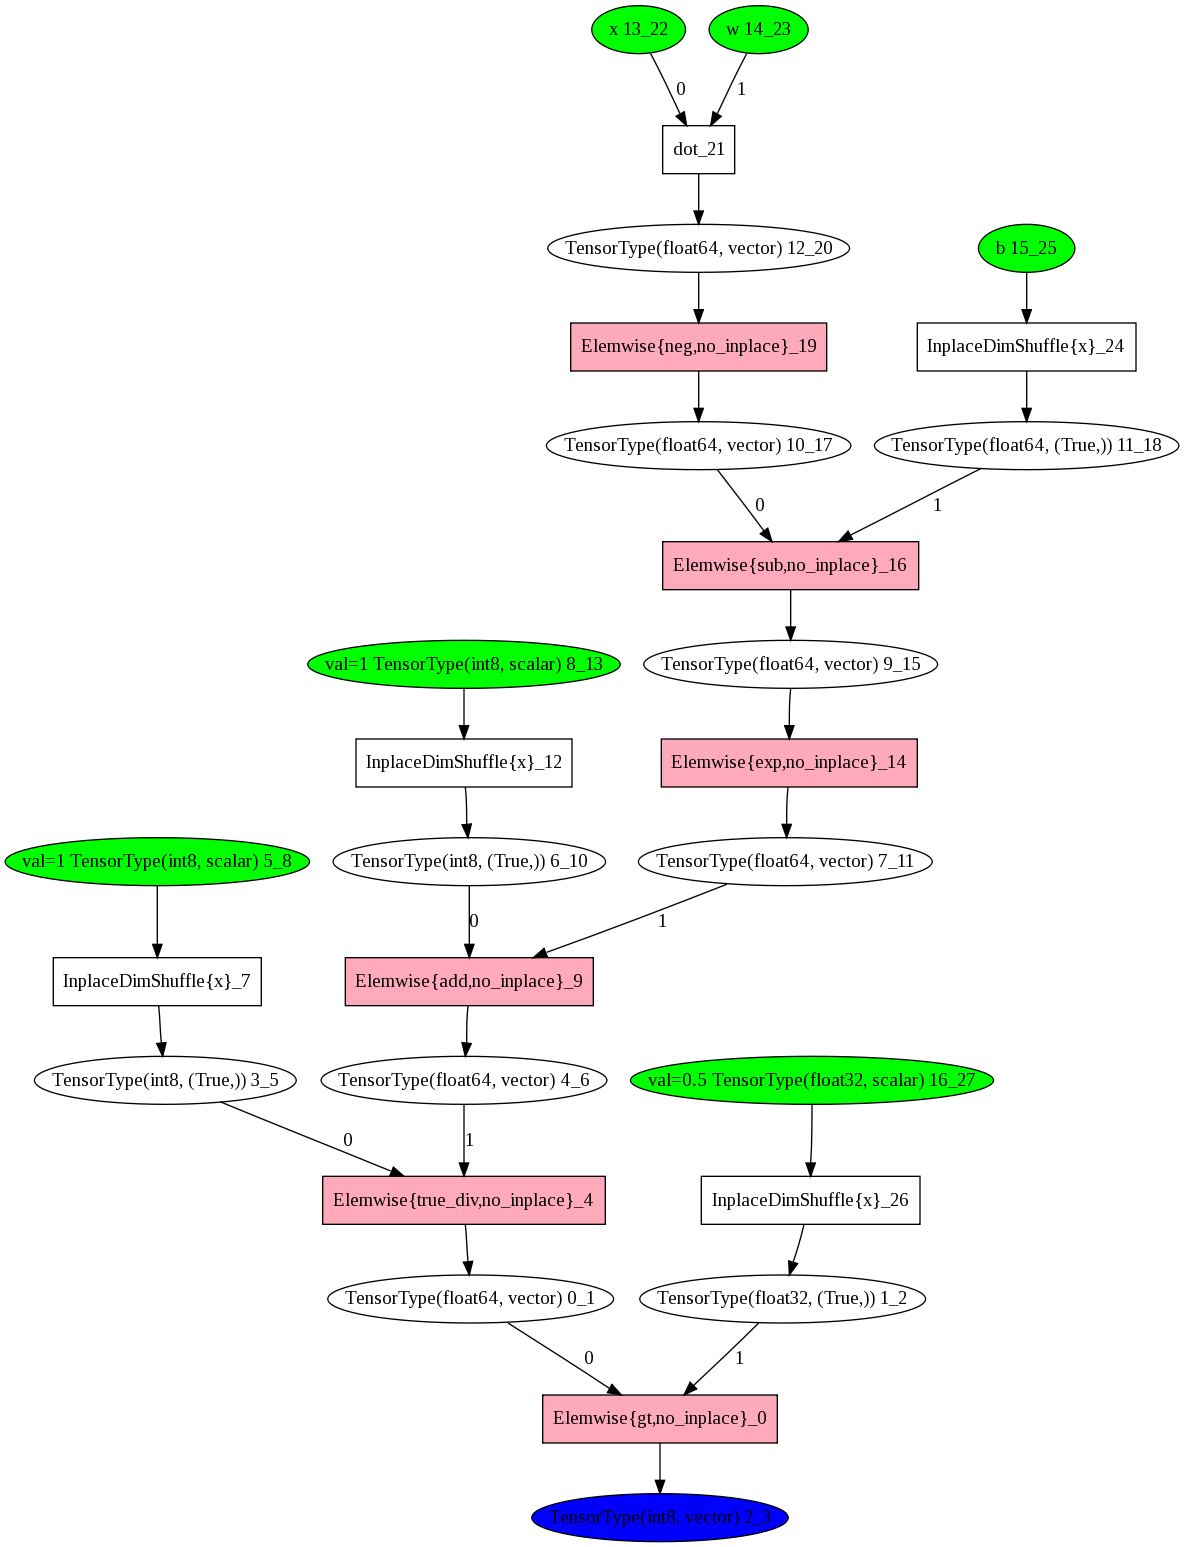
\includegraphics[width=1.9in]{pics/logreg_pydotprint_prediction.png}
\end{frame}

\begin{frame}[fragile]
\frametitle{Picture Printing of Graphs}
\begin{Verbatim}
All pydotprint* requires graphviz and pydot
>>> theano.printing.pydotprint(predict)
\end{Verbatim}
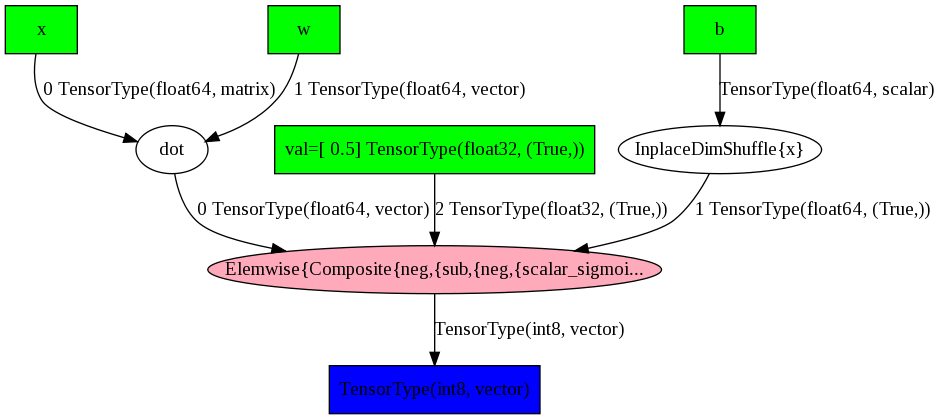
\includegraphics[width=4in]{pics/logreg_pydotprint_predic.png}
\end{frame}

\begin{frame}[fragile]
\frametitle{Picture Printing of Graphs}
\begin{Verbatim}[commandchars=\\\{\}]
>>> theano.printing.pydotprint(train) {\color{gray}# This is a small train example!}
\end{Verbatim}
\hspace{-.8cm}
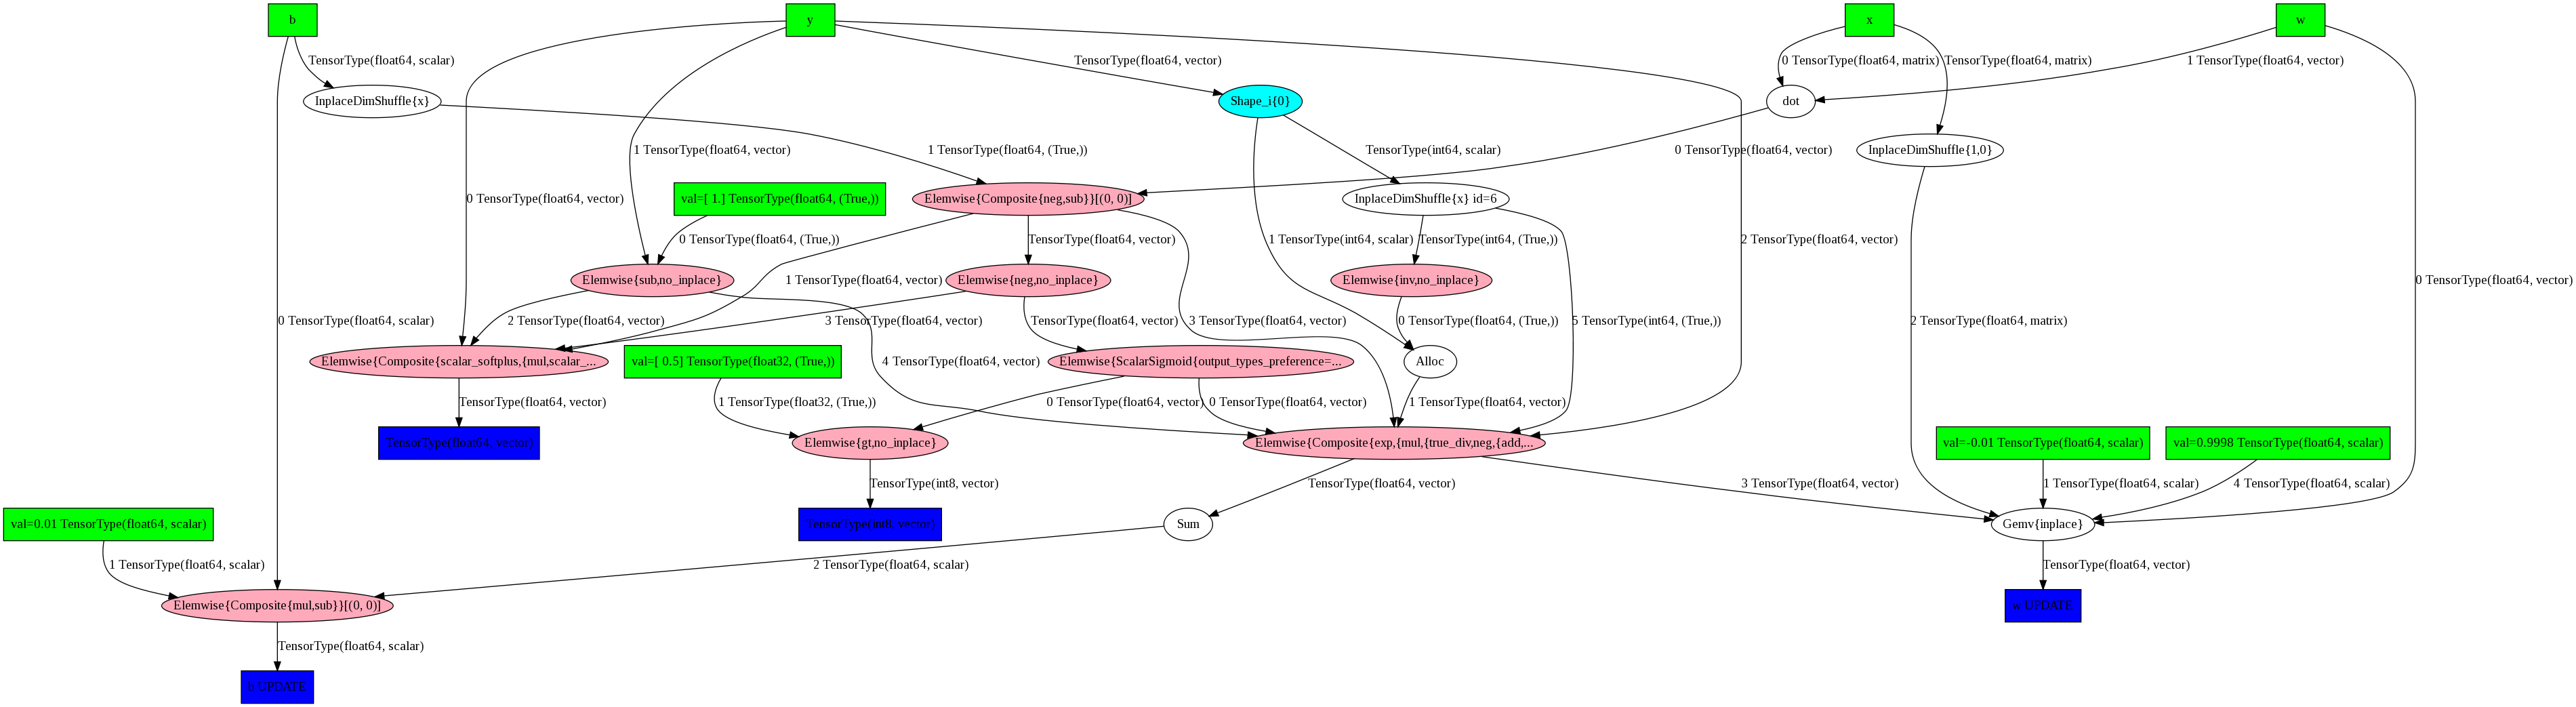
\includegraphics[width=5.0in]{pics/logreg_pydotprint_train.png}
\end{frame}


\subsection{Debugging}
\frame{
\frametitle{How to Debug}
\begin{itemize}
\item Run with the flag \texttt{mode=DebugMode}
  \begin{itemize}
  \item 100-1000x slower
  \item Test all optimization steps from the original graph to the final graph
  \item Checks many things that Op should/shouldn't do
  \item Executes both the Python and C code versions
  \end{itemize}
\item Run with the Theano flag \texttt{compute\_test\_value = {``off'', ``ignore'', ``warn'', ``raise''}}
  \begin{itemize}
  \item Run the code as we create the graph
  \item Allows you to find the bug earlier (ex: shape mismatch)
  \item Makes it easier to identify where the problem is in \textit{your} code
  \item Use the value of constants and shared variables directly
  \item For pure symbolic variables uses \texttt{x.tag.test\_value = numpy.random.rand(5,10)}
  \end{itemize}
\item Run with the flag \texttt{mode=FAST\_COMPILE}
  \begin{itemize}
  \item Few optimizations
  \item Run Python code (better error messages and can be debugged \\ interactively in the Python debugger)
  \end{itemize}
\end{itemize}
}

\subsection{Loops}
\frame{
\frametitle{Scan}
\begin{itemize}
\item General form of {\bf recurrence}, which can be used for looping.
\item {\bf Reduction} and {\bf map}(loop over the leading dimensions) are special cases of Scan
\item You *scan* a function along some input sequence, producing an
  output at each time-step
\item The function can see the {\bf previous K time-steps} of your function
\item ``sum()`` could be computed by scanning the $z + x_i$ function
  over a list, given an initial state of ``z=0``.
\item Often a for-loop can be expressed as a ``scan()`` operation, and
  ``scan`` is the closest that Theano comes to looping. 
\item The advantage of using ``scan`` over for loops
  \begin{itemize}
  \item The number of iterations to be part of the symbolic graph
  \item Minimizes GPU transfers if GPU is involved
  \item Compute gradients through sequential steps
  \item Slightly faster then using a for loop in Python with a compiled Theano function 
  \item Can lower the overall memory usage by detecting the actual \\ amount of memory needed
  \end{itemize}
\end{itemize}
}

\begin{frame}[fragile]
\frametitle{Scan Example: Computing pow(A,k)}
\begin{Verbatim}
k = T.iscalar("k"); A = T.vector("A")

def inner_fct(prior_result, A): return prior_result * A
# Symbolic description of the result
result, updates = theano.scan(fn=inner_fct,
                              outputs_info=T.ones_like(A),
                              non_sequences=A, n_steps=k)

# Scan has provided us with A**1 through A**k.  Keep only the last
# value. Scan notices this and does not waste memory saving them.
final_result = result[-1]

power = theano.function(inputs=[A,k], outputs=final_result,
                        updates=updates)

print power(range(10),2)
#[  0.   1.   4.   9.  16.  25.  36.  49.  64.  81.]
\end{Verbatim}
\end{frame}

\begin{frame}[fragile]
\frametitle{Scan Example: Calculating a Polynomial}
\begin{Verbatim}
coefficients = theano.tensor.vector("coefficients")
x = T.scalar("x"); max_coefficients_supported = 10000

# Generate the components of the polynomial
full_range=theano.tensor.arange(max_coefficients_supported)
components, updates = theano.scan(fn=lambda coeff, power, free_var: 
                                     coeff * (free_var ** power),
                                  outputs_info=None,
                                  sequences=[coefficients, full_range],
                                  non_sequences=x)
polynomial = components.sum()
calculate_polynomial = theano.function(inputs=[coefficients, x],
                                       outputs=polynomial)

test_coeff = numpy.asarray([1, 0, 2], dtype=numpy.float32)
print calculate_polynomial(test_coeff, 3)
# 19.0
\end{Verbatim}
\end{frame}

\frame{
\frametitle{Exercises 5}
\begin{itemize}
\item Run the example in the file scan\_pow.py and scan\_poly.py
\item Modify and execute the polynomial example to have the reduction done by scan
\end{itemize}
}

\frame{
\frametitle{Known Limitations}
\begin{itemize}
\item Compilation phase distinct from execution phase
\item Compilation time can be significant
  \begin{itemize}
  \item Amortize it with functions over big input or reuse functions
  \end{itemize}
\item Execution overhead
  \begin{itemize}
  \item Needs a certain number of operations to be useful
  \item We have started working on this in a branch
  \end{itemize}
\item Compilation time superlinear in the size of the graph. 
  \begin{itemize}
  \item A few hundreds nodes is fine
  \item Disabling a few optimizations can speed up compilation
  \item Usually too many nodes indicates a problem with the graph
  \end{itemize}
\item Lazy evaluation in a branch (We will try to merge this summer)
\end{itemize}

}

\section{PyCUDA}
\subsection{PyCUDA}

\begin{frame}[fragile]
\frametitle{PyCUDA}
\begin{center}
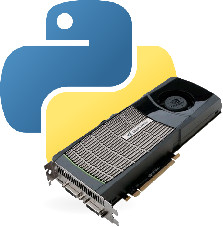
\includegraphics[width=2.5in]{pics/pycuda-logo-crop.pdf}
\end{center}
\end{frame}


\frame{
\frametitle{Intro}
Authors: Andreas Kl\"{o}ckner

\begin{itemize}
\item PyCUDA can access Nvidia's CUDA parallel computation API from Python
\item Object cleanup tied to lifetime of objects (RAII, Resource Acquisition Is Initialization).
  \begin{itemize}
  \item Makes it much easier to write correct, leak- and crash-free code
  \item PyCUDA knows about dependencies (e.g.. it won't detach from a context before all memory allocated in it is also freed)
  \end{itemize}
\item Convenience
  \begin{itemize}
  \item Abstractions to compile CUDA code from Python: \texttt{pycuda.driver.SourceModule}
  \item A GPU memory buffer: \texttt{pycuda.gpuarray.GPUArray}
  \end{itemize}
\item Completeness
  \begin{itemize}
  \item Binding to all of CUDA's driver API
  \end{itemize}
\item Automatic Error Checking
  \begin{itemize}
  \item All CUDA errors are automatically translated into Python exceptions
  \end{itemize}
\item Speed
  \begin{itemize}
  \item PyCUDA's base layer is written in C++
  \end{itemize}
\item Helpful documentation
\end{itemize}

}

\begin{frame}[fragile]
\frametitle{Example}
\begin{Verbatim}
import pycuda.autoinit
import pycuda.driver as drv
import numpy

from pycuda.compiler import SourceModule
mod = SourceModule("""
__global__ void multiply_them(float *dest, float *a, float *b)
{
  const int i = threadIdx.x;
  dest[i] = a[i] * b[i];
}
""")

\end{Verbatim}
\end{frame}

\begin{frame}[fragile]
\frametitle{Example}
\begin{Verbatim}
multiply_them = mod.get_function("multiply_them")

a = numpy.random.randn(400).astype(numpy.float32)
b = numpy.random.randn(400).astype(numpy.float32)

dest = numpy.zeros_like(a)
multiply_them(
        drv.Out(dest), drv.In(a), drv.In(b),
        block=(400,1,1), grid=(1,1))
\end{Verbatim}
\end{frame}

%\frame{
%\frametitle{GpuArray}
%TODO: No support for strided memory.
%}

\section{CUDA}
\subsection{CUDA Overview}
\frame{
\frametitle{GPU Programming: Gains and Losses}
\begin{itemize}
\item Gains:
\begin{itemize}
\item Memory Bandwidth (140GB/s vs 12 GB/s)
\item Compute Bandwidth( Peak: 1 TF/s vs 0.1 TF/s in float)
\item Data-parallel programming
\end{itemize}

\item Losses:
\begin{itemize}
\item No performance portability guaranty
\item Data size influence more the implementation code on GPU
\item Cheap branches
\item Fine-grained malloc/free*
\item Recursion*
\item Function pointers*
\item IEEE 754FP compliance*
\end{itemize}
\end{itemize}

* Less problematic with new hardware (NVIDIA Fermi)

\small{\color{gray}[slide from Andreas Kl\"{o}ckner]}
}

\frame{
\frametitle{CPU vs GPU Architecture}
%\begin{center}
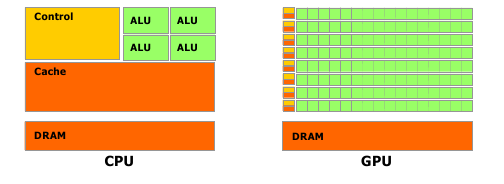
\includegraphics[width=4.7in]{pics/CPU_VS_GPU.png}

\small{\color{gray}Source NVIDIA CUDA\_C\_Programming\_Guide.pdf document}
%\end{center}
}

\frame{
\frametitle{Different GPU Block Repartition}
\begin{center}
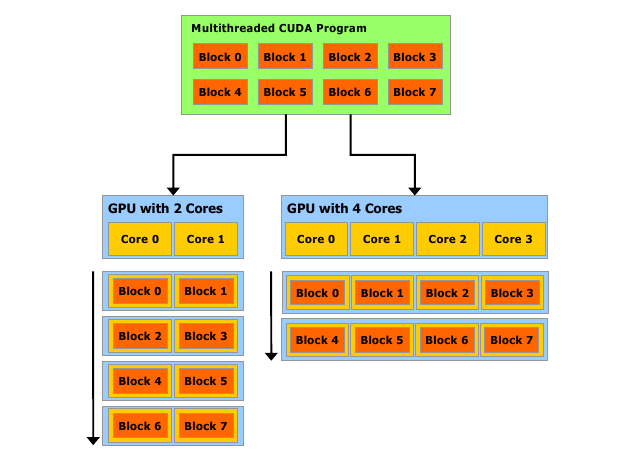
\includegraphics[width=3.2in]{pics/bloc_repartition.png}

\small{\color{gray}Source NVIDIA CUDA\_C\_Programming\_Guide.pdf document}
\end{center}
}

\frame{
\frametitle{GPU thread structure}
\begin{center}
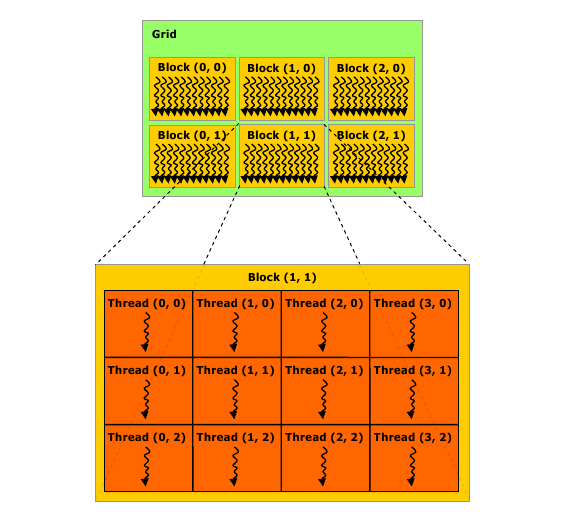
\includegraphics[width=2.7in]{pics/grid_block_thread.png}

\small{\color{gray}Source NVIDIA CUDA\_C\_Programming\_Guide.pdf document}
\end{center}
}

\begin{frame}
\frametitle{Exercises 6}
\begin{itemize}
\item Run the example in the file pycuda\_simple.py
\item Modify and execute it to work for a matrix of 20 $\times$ 10
\end{itemize}
\end{frame}

%\begin{frame}
%\frametitle{PyCUDA Exercises:TODO MOVE?!?!?}
%\begin{itemize}
%\item Run the example
%\item Modify it to multiple two matrix (rename it to MulMatrix)
%\item Modify it to multiple two inputs with arbitrary number of dimensions
%\end{itemize}
%\end{frame}


\section{Extending Theano}
\subsection{Theano}
\frame{
\frametitle{Theano Graph}
\begin{itemize}
\item Theano works with symbolic graphs
\item Those graphs are bi-partite graphs (graph with 2 types of nodes)
\item Those 2 nodes types are Apply and Variable nodes
\end{itemize}
\begin{itemize}
\item Inputs and Outputs are lists of Theano variables
\end{itemize}
\begin{center}
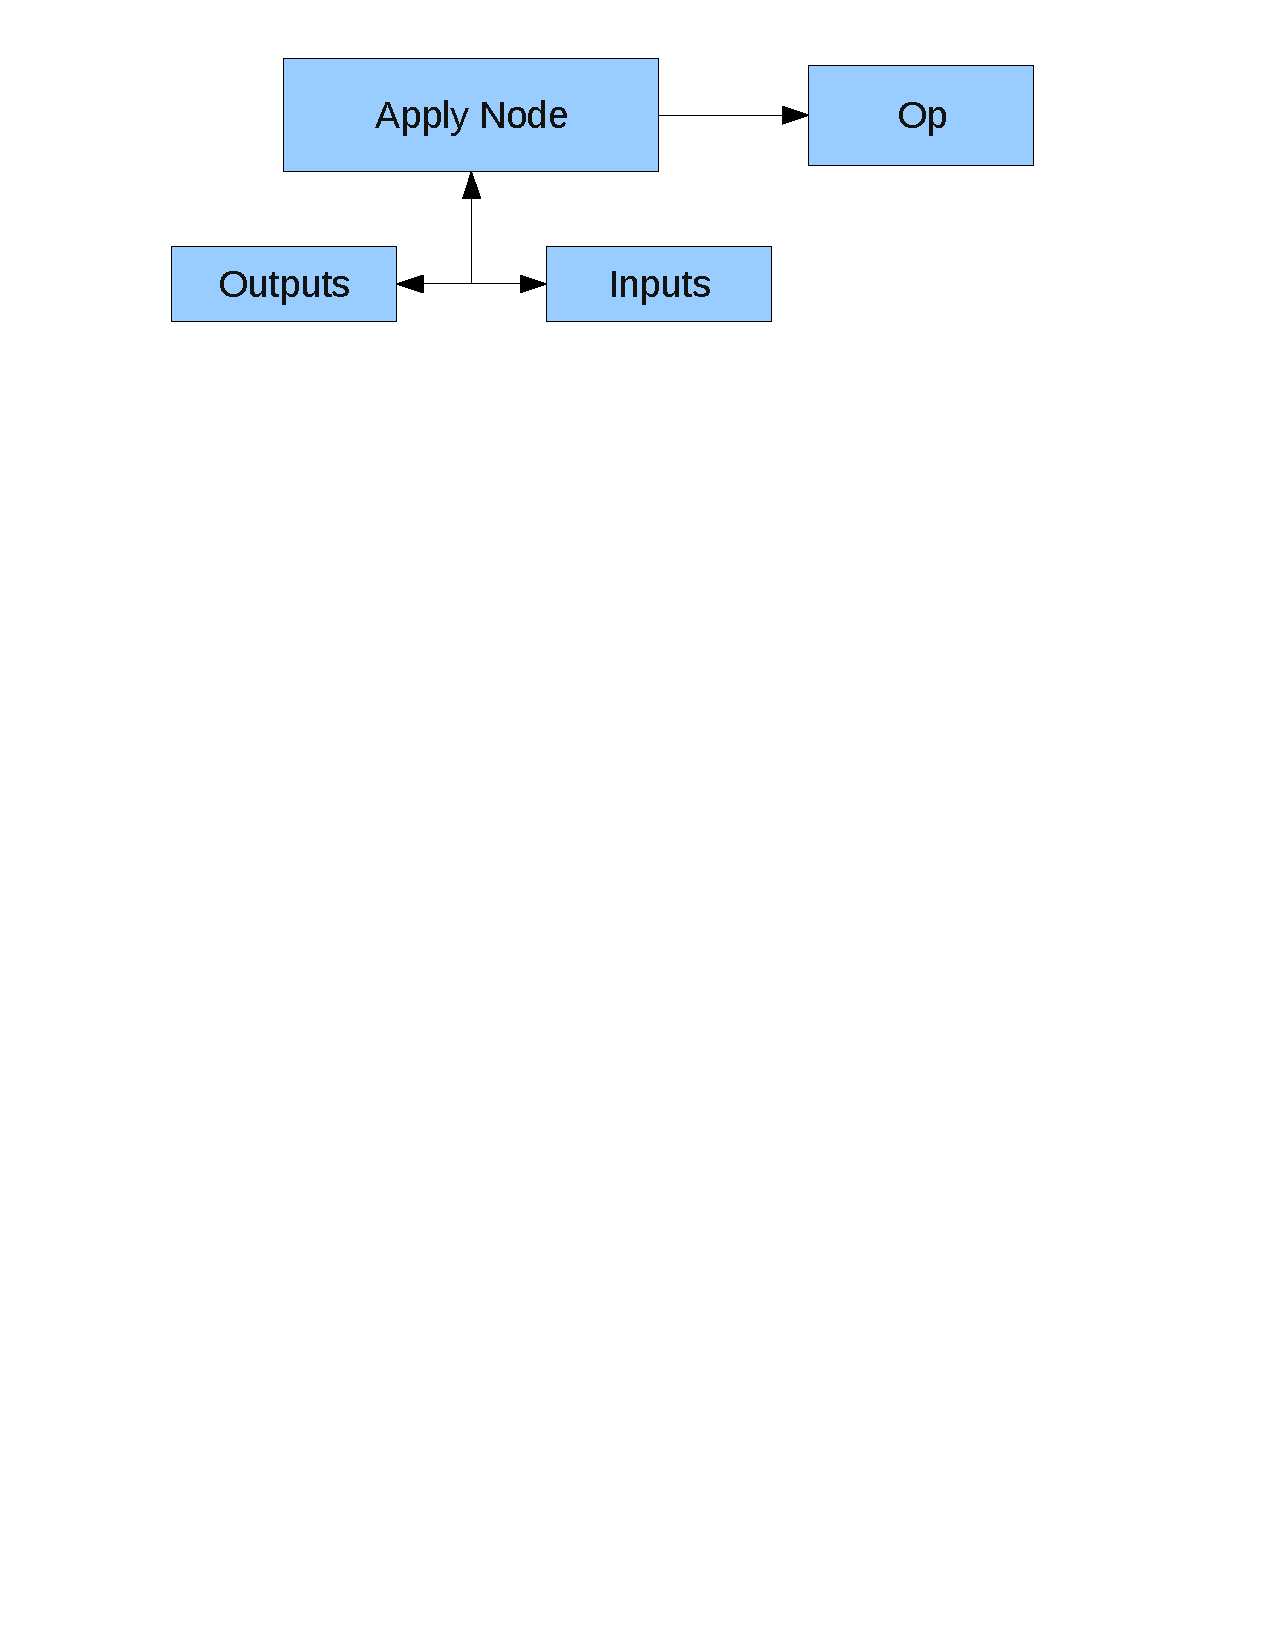
\includegraphics[width=3.5in]{pics/apply_node.pdf}
\end{center}
}

\begin{frame}[fragile]
\frametitle{Op Contract}
\begin{Verbatim}[commandchars=\\\{\}]
class MyOp(Op):
    def __eq__(self, other):
    def __hash__(self):
    def __str__(self):
    def make_node(self, *inputs):

{\color{gray}# Python implementation:}
    def perform(self, node, inputs_storage, outputs_storage):
{\color{gray}# C implementation:} [see theano web site]
{\color{gray}# others implementation (pycuda, ...):}
     def make_thunk(self, node, storage_map, _, _2):

{\color{gray}# optional:}
    def __init__(self, ...):
    def grad(self, inputs, g):
    def infer_shape(node, (i0_shapes, ...))
\end{Verbatim}
\end{frame}

\begin{frame}[fragile]
\frametitle{Op Example}
\begin{Verbatim}
import theano

class DoubleOp(theano.Op):
    def __eq__(self, other):
        return type(self) == type(other)
    def __hash__(self):
        return hash(type(self))
    def __str__(self):
        return self.__class__.__name__
    def make_node(self, x):
        x = theano.tensor.as_tensor_variable(x)
        return theano.Apply(self, [x], [x.type()])
    def perform(self, node, inputs, output_storage):
        x = inputs[0]
        z = output_storage[0]
        z[0] = x * 2

\end{Verbatim}
\end{frame}

\begin{frame}[fragile]
\frametitle{Theano Op Example: Test it!}
\begin{Verbatim}
x = theano.tensor.matrix()
f = theano.function([x],DoubleOp()(x))

import numpy
inp = numpy.random.rand(5,5)
out = f(inp)
assert numpy.allclose(inp*2, out)
print inp
print out
\end{Verbatim}
\end{frame}

\begin{frame}
\frametitle{Exercises 7}
\begin{itemize}
\item Run the code in the file double\_op.py.
\item Modify and execute to compute: $x * y$
\item Modify and execute the example to return 2 outputs: $x + y$ and $x - y$
  \begin{itemize}
  \item Our current elemwise fusion generate computation with only 1 outputs
  \end{itemize}
\end{itemize}
\end{frame}

\subsection{Theano+PyCUDA}
\begin{frame}[fragile]
\frametitle{Theano+PyCUDA Op Example}
\begin{Verbatim}
import numpy, theano
import theano.misc.pycuda_init
from pycuda.compiler import SourceModule
import theano.sandbox.cuda as cuda

class PyCUDADoubleOp(theano.Op):
    def __eq__(self, other):
        return type(self) == type(other)
    def __hash__(self):
        return hash(type(self))
    def __str__(self):
        return self.__class__.__name__
    def make_node(self, inp):
        inp = cuda.basic_ops.gpu_contiguous(
           cuda.basic_ops.as_cuda_ndarray_variable(inp))
        assert inp.dtype == "float32"
        return theano.Apply(self, [inp], [inp.type()])
\end{Verbatim}
\end{frame}


\begin{frame}[fragile]
\frametitle{Theano + PyCUDA Op Example: make\_thunk}
\begin{Verbatim}
    def make_thunk(self, node, storage_map, _, _2):
        mod = SourceModule( THE_C_CODE )

        pycuda_fct = mod.get_function("my_fct")
        inputs = [ storage_map[v] for v in node.inputs]
        outputs = [ storage_map[v] for v in node.outputs]
        def thunk():
            z = outputs[0]
            if z[0] is None or z[0].shape!=inputs[0][0].shape:
                z[0] = cuda.CudaNdarray.zeros(inputs[0][0].shape)
            grid = (int(numpy.ceil(inputs[0][0].size / 512.)),1)
            pycuda_fct(inputs[0][0], z[0], numpy.intc(inputs[0][0].size),
                       block=(512,1,1), grid=grid)
        return thunk
\end{Verbatim}
\end{frame}

\begin{frame}[fragile]
\frametitle{Theano + PyCUDA Op Example: GPU Code}
\begin{Verbatim}
THE_C_CODE = """
__global__ void my_fct(float * i0, float * o0, int size) {
    int i = blockIdx.x*blockDim.x + threadIdx.x;
    if(i<size){
        o0[i] = i0[i]*2;
    }
}""")
\end{Verbatim}
\end{frame}


\begin{frame}[fragile]
\frametitle{Theano + PyCUDA Op Example: Test it!}
\begin{Verbatim}
x = theano.tensor.fmatrix()
f = theano.function([x], PyCUDADoubleOp()(x))
xv=numpy.ones((4,5), dtype="float32")

assert numpy.allclose(f(xv), xv*2)
print numpy.asarray(f(xv))
\end{Verbatim}
\end{frame}

\begin{frame}
\frametitle{Exercises 8}
\begin{itemize}
\item Run the example in the file pycuda\_double\_op.py
\item Modify and execute the example to multiple two matrix: $x * y$
\item Modify and execute the example to return 2 outputs: $x + y$ and $x - y$
  \begin{itemize}
  \item Our current elemwise fusion generate computation with only 1 outputs
  \end{itemize}
\item Modify and execute the example to support stride? (Don't force the input to be c contiguous)
\end{itemize}
\end{frame}

\section{GpuNdArray}
\subsection{GpuNdArray}
\frame{
\frametitle{Why a common GPU ndarray?}
\begin{itemize}
\item Currently there are at least 4 different GPU array data structures in use by Python packages
  \begin{itemize}
  \item CudaNdarray (Theano), GPUArray (PyCUDA), CUDAMatrix (cudamat), GPUArray (PyOpenCL), ...
  \item There are even more if we include other languages
  \end{itemize}
\item All of them are a subset of the functionality of \texttt{numpy.ndarray} on the GPU
\item Lots of duplicated effort
  \begin{itemize}
  \item GPU code is harder/slower to do {\bf correctly} and {\bf fast} than on the CPU/Python
  \end{itemize}
\item Lack of a common array API makes it harder to port/reuse code
\item Also harder to find/distribute code
\item Divides development work
\end{itemize}

}

\frame{
\frametitle{Design Goals}
\begin{itemize}
\item Make it VERY similar to \texttt{numpy.ndarray}
\item Be compatible with both CUDA and OpenCL
\item Have the base object accessible from C to allow collaboration with more projects, across high-level languages
  \begin{itemize}
  \item We want people from C, C++, Ruby, R, ... all use the same base GPU N-dimensional array
  \end{itemize}
\end{itemize}
}

\frame{
\frametitle{Final GpuNdArray Note}
\begin{itemize}
\item Under development
\item Will be the next GPU array container for Theano (this summer!)
\item Probably also for PyCUDA, PyOpenCL
\item Mailing list: http://lists.tiker.net/listinfo/gpundarray
\end{itemize}

}

\section{Conclusion}
\subsection{Conclusion}
\frame{
  \frametitle{Conclusion}
  \begin{itemize}
  \item I presented a tool that tries to be the holy grail in computing: {\bf easy to code} and {\bf fast to execute}!
  \item Generates fast, custom CPU code \textit{and} GPU code
  \item You can easily wrap existing CPU/GPU code with Theano
  \item It {\bf works} and is {\bf used in the real world} by academic researchers \textit{and} industry 
  \end{itemize}
}

\frame{
  \frametitle{Thanks}
  \begin{itemize}
  \item Thanks for attending this tutorial
    \vfill
  \item Thanks to our agencies that resources for this projects: Calcul Qu\'ebec, CIFAR, Compute Canada, FQRNT, MITACS, NSERC, SciNet, SHARCNET, Ubisoft and WestGrid.
  \end{itemize}
}

\frame{
%  \frametitle{}
\center{\huge{Questions/Comments?}}
}

\end{document}
